\subsection{Independent Factorization on Lexical-Anchoring}
\label{ssec:lex-phr:lex-factorization-analysis}
In the following, we focus on the first two main challenges in
independent factorization: \textbf{output decomposition} and
\textbf{input decomposition} on lexical-anchoring. We leave the
\textbf{factor modelling} into the next part.  We take a more
complicated AMR graph in~\autoref{fig:bg:amr} as an example, for the
sentence, \kw{Pierre Vinken, 61 years old, will join the board as a
  nonexecutive director Nov.29.} We introduce the details of
independent factorization for AMR and other lexical-anchoring
representations.

%\begin{figure}[t]
%\centering
%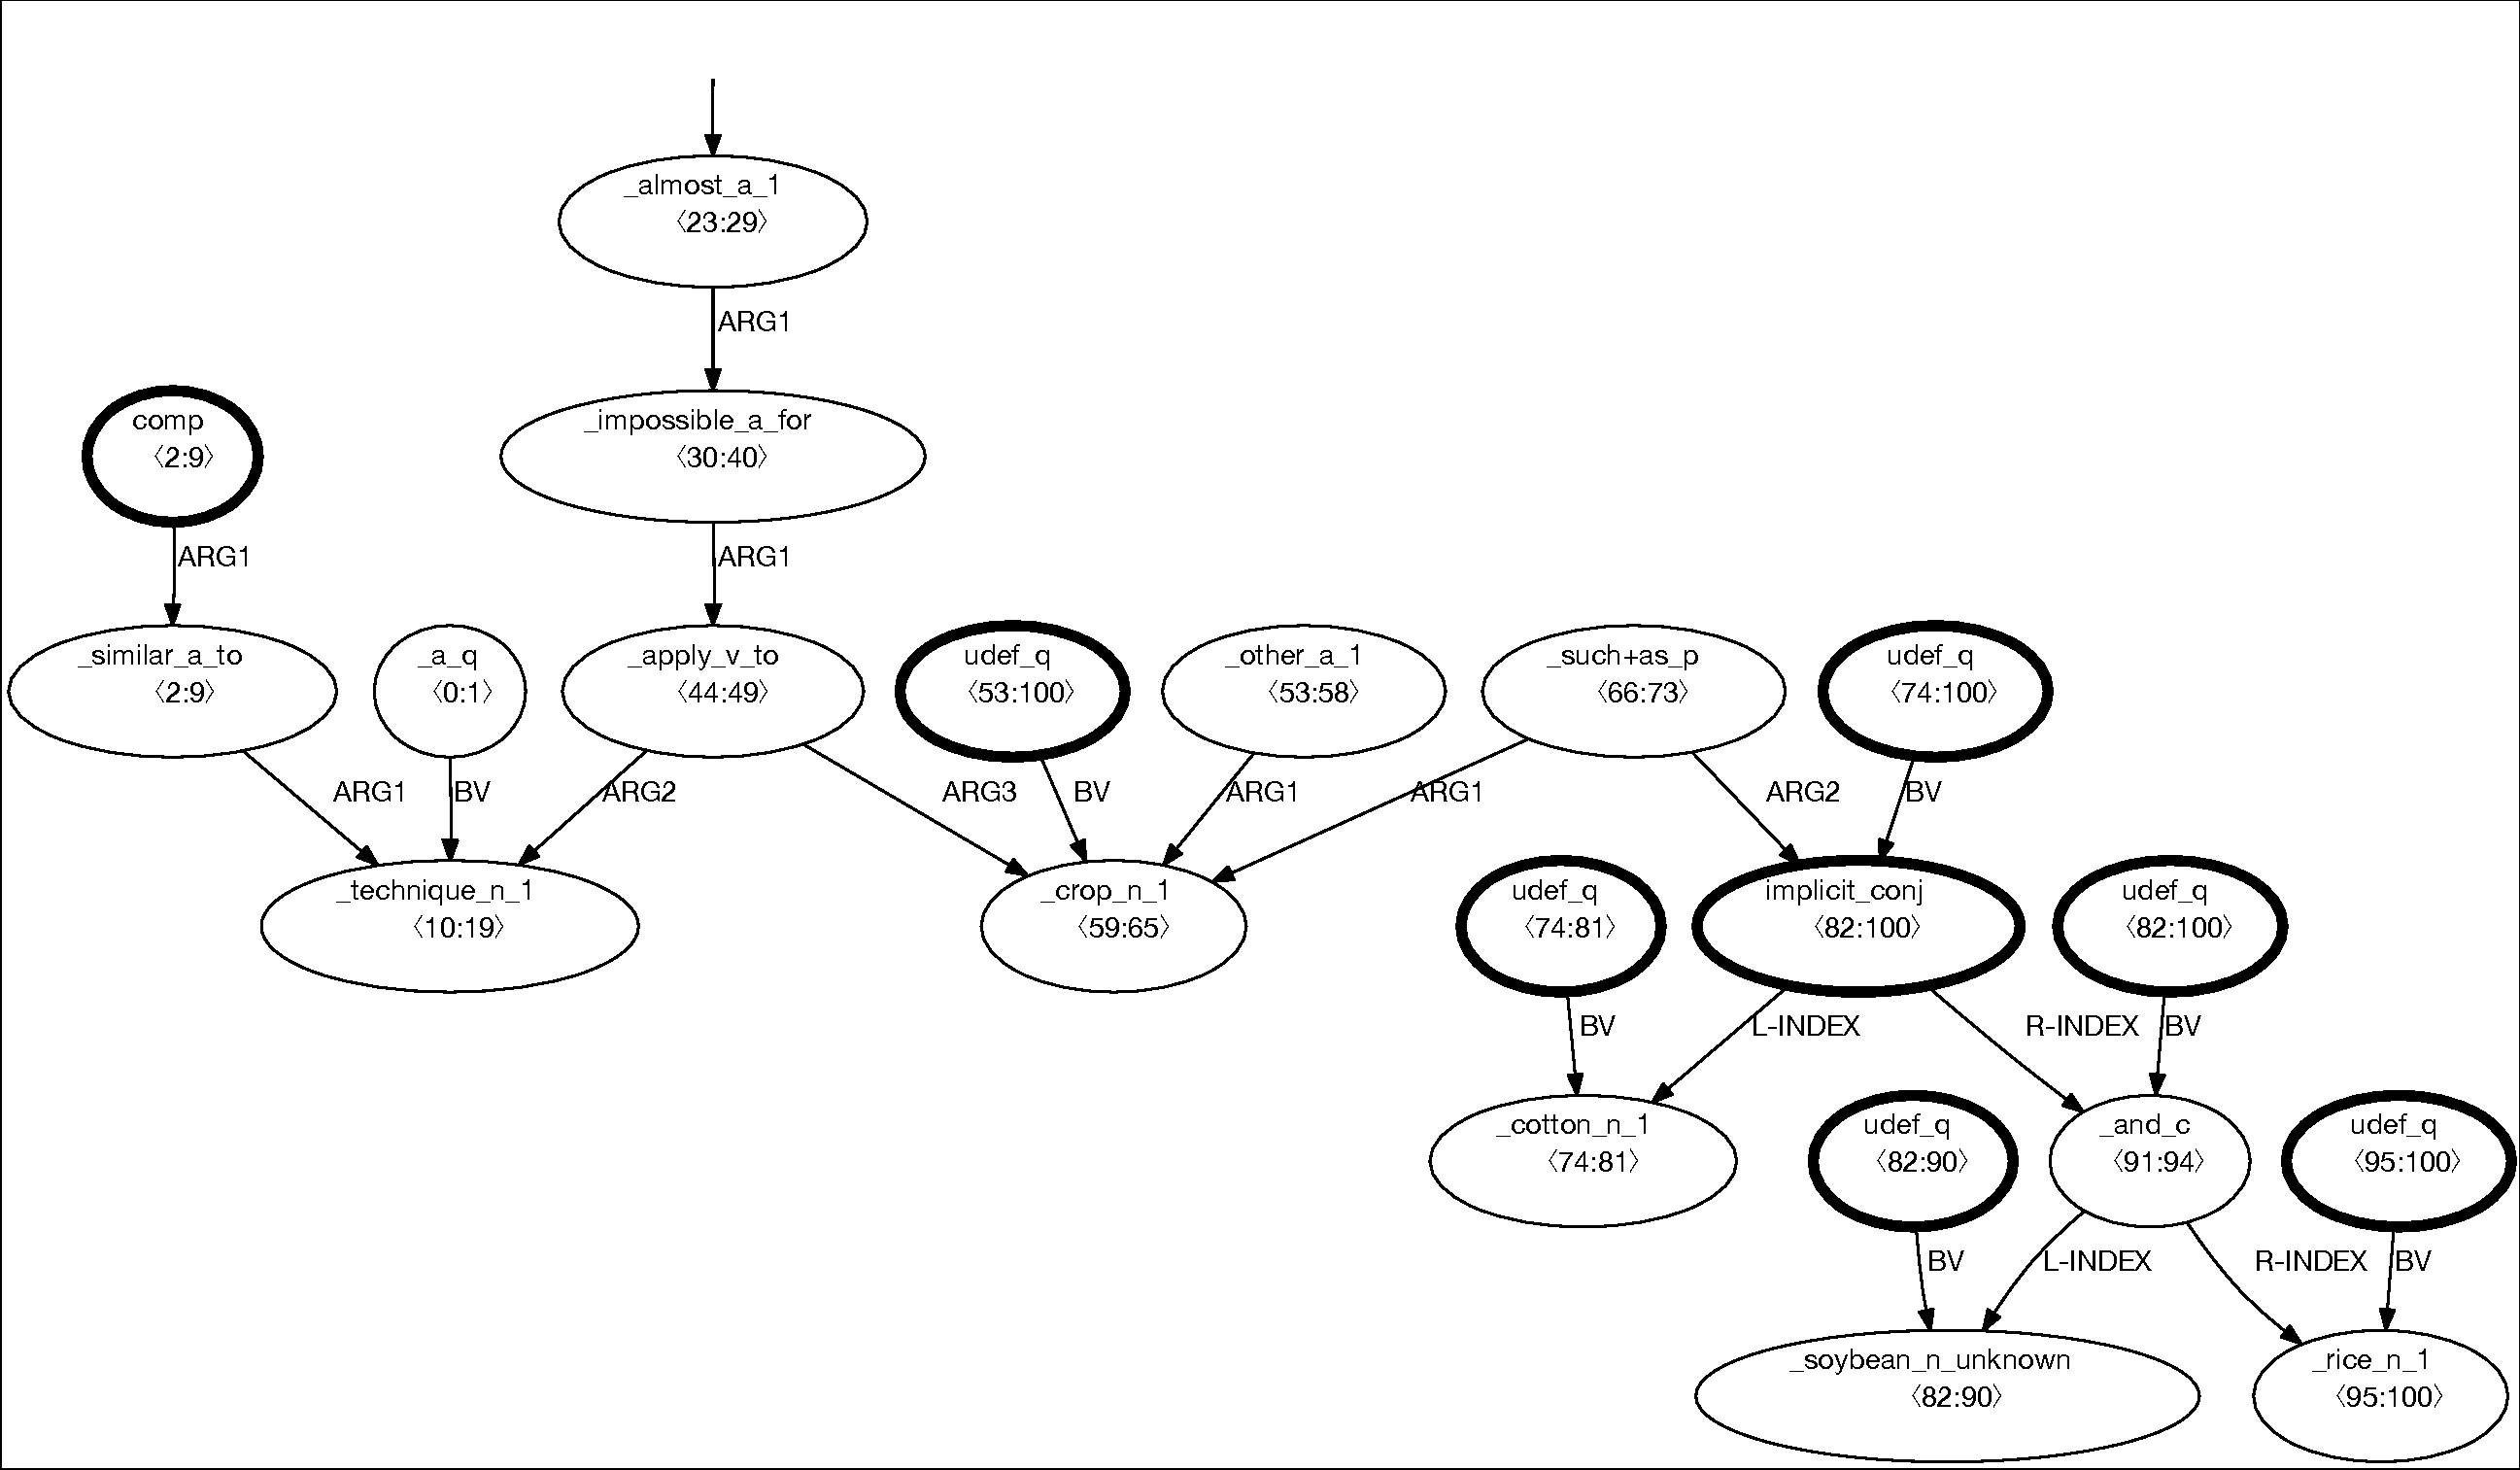
\includegraphics[width=.96\textwidth,trim=.1cm .1cm .05cm .05cm, clip]{eds-white.pdf}
%\caption{\label{fig:phrasal-anchoring}Phrasal-anchoring in
%  EDS[wsj\#0209013], for the sentence \texttt{\char`\"A similar
%    technique is almost impossible to apply to other crops, such as
%    cotton, soybeans and rice.\char`\"}. Bold nodes are similar to the
%  non-terminal nodes in UCCA, which are anchored multiple tokens, thus
%  overlapping with the anchors of other nodes.}
%\end{figure}

\subsubsection{Output Decomposition}
\label{sssec:lex-phr:lex-output-decomposition}
For the lexical-anchoring graph-based representations~(DM, PSD, AMR),
the target graph can be decomposed into independent nodes or
subgraphs. For DM and PSD, each node in the target graph is strictly
aligned to the corresponding token. Hence, we simply decompose the DM
and PSD graph by nodes. However, when we introduce the necessary of
structural inductive biases for independent
factorization~(\autoref{sssec:intro:structural-biases}), the AMR
parsing running examples shows that we need to handle those special
entities in AMR graph.  From the training data alone, we cannot easily
tell how to segment the AMR graphs. However, according to the
annotation guideline of AMR and previous work on subgraph
templating~\cite{Werling:2015up} or abstract concept
label~\cite{Wang:2017vt}, the main intuition of grouping is to ensure
that concepts are rarely lexically triggered (e.g., \tquoted{person}
and \dquoted{have-org-role-91} in~\autoref{fig:bg:amr} get grouped
together with lexically triggered nodes~(e.g., \tquoted{Pierre
  Vinken}, and \dquoted{director}). Finally, we adopt the templates
proposed by~\citet{corro2019learning} including:
\tquoted{thing}~(e.g., \tquoted{(opine-01 :ARG-01 thing)} for
\tquoted{opinion}), \tquoted{person}~(e.g., \tquoted{(play-01 :ARG1
  person)} for \tquoted{player}), \tquoted{more},
\tquoted{most}~(e.g., \tquoted{(have-degree-91 :ARG2 good-02) :ARG3
  more)} for \tquoted{better}),
\tquoted{date-entity}~(e.g.,\tquoted{(date-entity :month 2)} for
\tquoted{February}), and all the special quantity entities,
\tquoted{xx-quantity}~(e.g., \tquoted{(monetary-quantity :quant 20
  :unit dollar)} for \tquoted{\$20}).~\footnote{Please refer to the
  paper of~\citet{lyu2018amr} for more details about the recategorization.}

AMR output decomposition will be the rectangled segments shown in
\autoref{fig:lex-phr:amr-decomposition}.
\begin{figure}[!tbp]
  \centering
  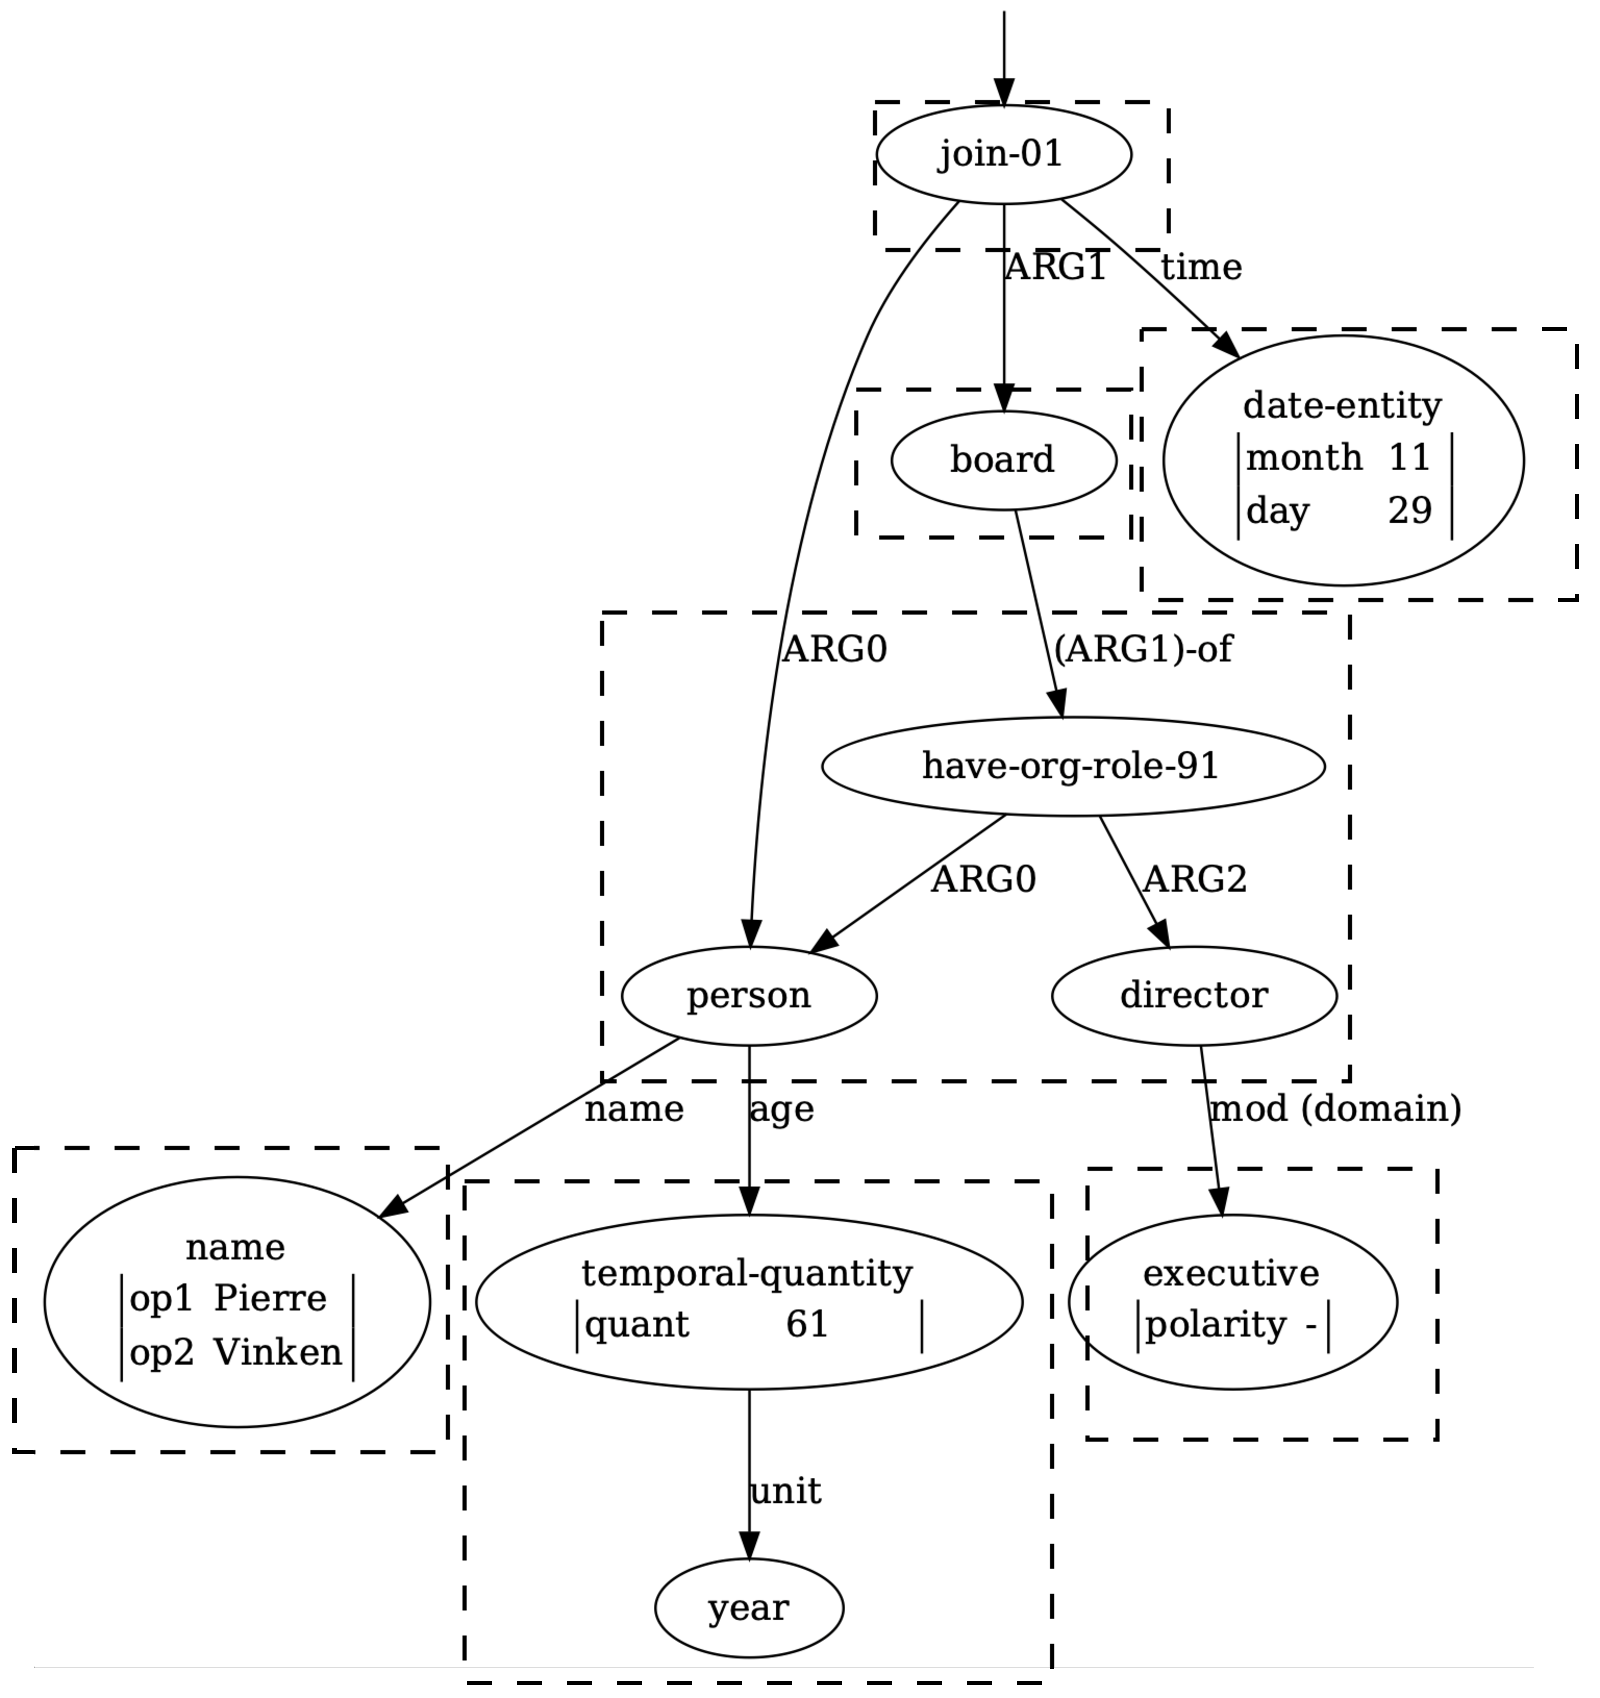
\includegraphics[width=0.90\textwidth]{pierre-decomposition.pdf}
  \caption{\label{fig:lex-phr:amr-decomposition} AMR output
    decomposition for the sentence \#20001001}
\end{figure}

\subsubsection{Input Decomposition and Alignments Discovery}
\label{sssec:lex-phr:lex-input-decomposition}

According to the bi-lexical dependency structures of DM and PSD, and
implicit lexical token anchoring on AMR, the nodes/categorized graph
fragments of DM, PSD, and AMR are anchored to surface lexical units in
an explicit or implicit way. Especially, those lexical units do not
overlap with each other, and most of them are just single-tokens,
multiple word expression, or named entities. In other words, when
parsing a sentence into DM, PSD, AMR graphs, and tokens in the original
sentence can be merged by looking up a lexicon dict when preprocessing
and then may be considered as a single token for aligning or parsing.

The more difficult challenge exists in how to align the decomposed
input with the decomposed output. According to the previous anchoring
analysis, the training data of DM and PSD naturally contains the
anchoring information, while the AMR training data doesn't offer the
alignments. Hence, for AMR, we need to an extra model to resolve the
alignments discovery problem. According to the AMR annotation
guideline, a strong inductive bias about the alignment is that
\emph{each token or expressive is not overlapping and is
  exclusively aligned to the output decompositions.} We will
introduce the details of the latent alignment model in
\autoref{ssec:lex-phr:latent-alignment}.

%%% Local Variables:
%%% mode: latex
%%% TeX-master: "../../dissertation-main.ltx"
%%% End:
